% ************************************
\section{Quantum Computing in a Nutshell}
% ************************************

\begin{frame}{Quantum Computing in a Nutshell}

\begin{columns}
 \column{0.6\linewidth}
    \begin{block}{Quantum register}
    $N$-qubit states $\ket\psi\in(\C^2)^{\otimes N}.$
    \end{block}
    
    \vspace{\floatsep}

    \begin{block}{Quantum circuit}
    Unitaries $U_1,\dots,U_L\in \SU(2^N)$
    \end{block}
    
    \vspace{\floatsep}
    
    \begin{block}{Measurement}
    $\Rightarrow$ computational result
    \end{block}
 
 \column{0.4\linewidth}
  \vspace{\floatsep}
    \Qcircuit @C=1em @R=1em {
      \lstick{\ket{q_1}} & \gate{U_1} & \qw & \multigate{1}{U_3} & \meter  \\
      \lstick{\ket{q_2}} & \qw & \multigate{1}{U_2} & \ghost{U_3} & \meter \\
      \lstick{\ket{q_3}} & \qw & \ghost{U_2} & \qw & \meter
    }
 
\end{columns}

\end{frame}

\begin{frame}{Quantum Algorithms}
 
 \structure{Hope/Expectation:} Many problems can be solved faster on a quantum computer.
 
 
 \begin{columns}
  \column{0.6\linewidth}
  \visible<2->{\structure{Evidence:}}
  \begin{itemize}
   \item<2-> Grover search
   \item<3-> Quantum Fourier Transform
   \item<3-> Shor's factorisation / discrete log 
   \item<4-> Topological Quantum Field Theory
   \item<4-> \dots
  \end{itemize}
  

  \column{0.4\linewidth}
    \begin{figure}
     \centering
     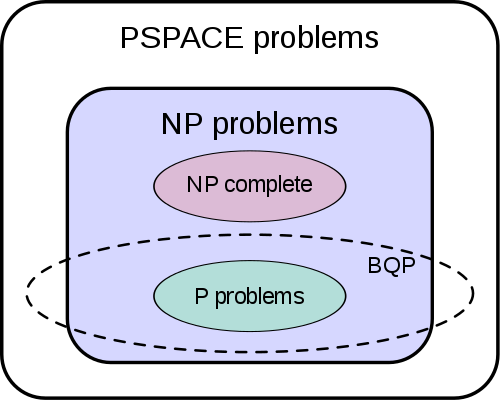
\includegraphics[width=\linewidth]{gfx/BQP_complexity_class_diagram}
     \caption{\footnotesize Wikipedia/BQP}
    \end{figure}
 \end{columns}
 
%  \begin{center}
%   \visible<5->{\alert{Number of quantum algorithms is very limited}}
%  \end{center}

\vspace{\floatsep}

\visible<5->{
\footnotesize{
\fullcite{brandao_quantum_2016}

\fullcite{van_apeldoorn_quantum_2017}
}
}
 
\end{frame}

